\addsection{Map Elements}{\images/logistics.png}

\begin{wrapfigure}{r}{0.5\textwidth}
  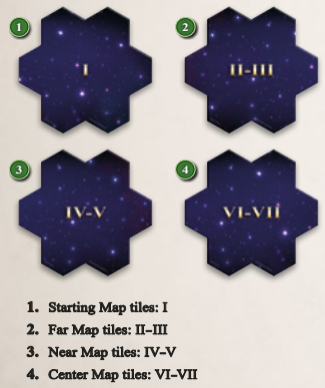
\includegraphics[width=0.9\linewidth]{\images/maptiles.png}
\end{wrapfigure}
Each scenario is built using four types of map tiles.
Players always have a faction-specific starting (I) map tile and may additionally have a number of face-down far (II-III) map tiles which can be used to add new areas to the scenario by spending MP.
Near (IV-V) and center (VI-VII) tiles are usually placed face down randomly during a scenario’s set up and must be turned face up by spending MP.\par
The roman numeral of each tile describes the overall difficulty of neutral armies on that tile, as well as the number of rewards players might expect to find on that tile.
Starting (I) tiles are the easiest while center (VI-VII) tiles are the most difficult.\par
During a scenario’s set up, you will be instructed to use a certain amount of specific map tiles.
Follow the scenario’s set up instructions and gather the necessary tiles.
All face-down tiles should be selected randomly from the pool of possible tiles and shuffled to keep their front side hidden.\par

\begin{wrapfigure}{R}{0.5\textwidth}
  \begin{center}
  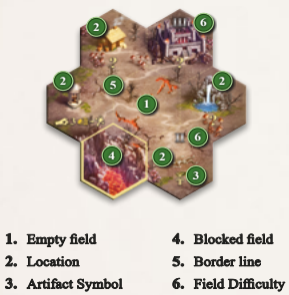
\includegraphics[width=0.47\textwidth]{\images/fields.png}
  \end{center}
\end{wrapfigure}
\subsection*{Map tile anatomy}
Each map tile is divided into 7 separate \textbf{fields} that your heroes can \textbf{visit}.
When a hero moves to a field, they must immediately visit it, or
first start a \hyperlink{Combat}{combat} against the enemies guarding it before visiting.
Empty fields do nothing when visited.
Solid yellow lines on a field's edge cannot be passed through.
\hyperlink{Difficulty}{Roman numerals} indicate that a field is guarded by neutral enemies that must be fought.\par

\clearpage

\subsection*{\hypertarget{Categories}{Location categories}}
Visiting fields provides heroes with benefits such as gaining resources or cards.
There are three categories of visitable fields:
\begin{itemize}
  \item \textbf{Visitable} – Once you visit this field, place a black cube on it.
    Treat it as an empty field as long as it has a black cube.
  \item \textbf{Flaggable} – These fields can be directly captured by players and provide passive benefits.
    When you visit it, place one of your faction cubes on it and gain a benefit.
    Enemy heroes who visit your flagged fields will replace your cube with theirs to steal the field’s effects.
    Allied heroes treat flagged fields as if they were empty.
  \item \textbf{Revisitable} – You can visit this field multiple times.
    Do not place a black cube when you visit it.
    You may pay 1 MP to visit this field again when your hero occupies this field.
\end{itemize}

See \hyperlink{All}{this section} for a list of all possible fields and what they do.
\subsection*{\hypertarget{Placing}{Placing and discovering new tiles}}
When you hero is adjacent to an undiscovered face down tile, that hero may spend 1 MP during your turn to turn that tile over.
You may then rotate the tile as you see fit and place it face-up.\par
In some scenarios you will receive your own individual stack of far (II-III) map tiles.
These can be placed on the map to expand the play area.
Tiles should be kept hidden from everyone until they are about to be placed.\par
Placing a new tile costs 1MP.
The new tile must be adjacent to the hero who spends the MP, and to at least two other existing tiles.
New tiles must also be positioned so that there is a valid path that eventually joins them with all other tiles.
You may always rotate map tiles when placing them.\par
\begin{center}
  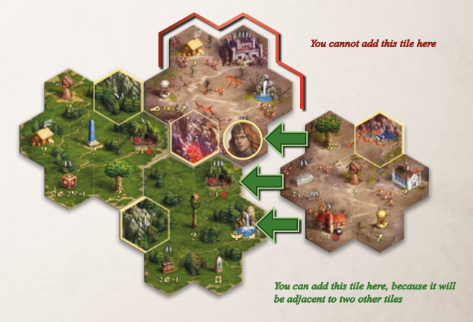
\includegraphics[width=\textwidth]{\images/placement.png}
\end{center}
